% Matteo Kumar
% PPB2 AFM
%Grundlagen

\chapter{Grundlagen}
\section{Aufbau und Funktionsweise}
Im Gegensatz zu optischen Mikroskopen basiert die Rasterkraftmikroskopie (atomic force microscopy, kurz AFM) auf der Detektion von Kräften. 
Hauptbestandteil sind eine Feder (Cantilever) und eine sehr feine, im Idealfall einatomige, Spitze. Mit dieser wird die Probe abgerastert 
(wie genau, siehe \ref{sec:Modi}). Dabei existieren eine Fülle an anziehenden und abstoßenden Kräften zwischen Probe und Spitze, beispielsweise 
Londonsche Dispersionskräfte oder Coulomb-Wechselwirkungen. Die Gesamtheit dieser Wechselwirkungen kann mit dem Lennard-Jones-Potential 
angenähert werden. Dieses ist, in Abhängigkeit vom Abstand $r$ zwischen den Molekülen, mit molekülabhängigen Parametern $a$, $b$: 
\begin{equation*}
    \Phi_{LJ}(r) = \frac{a}{r^{12}} - \frac{b}{r^6}
\end{equation*}
(\cite{Demtroeder2013}, S.126f) \\
Eine Skizze des Potentials ist in Abb. \ref{bild:LJP} zu sehen.

\begin{figure}[h]
    \centering
    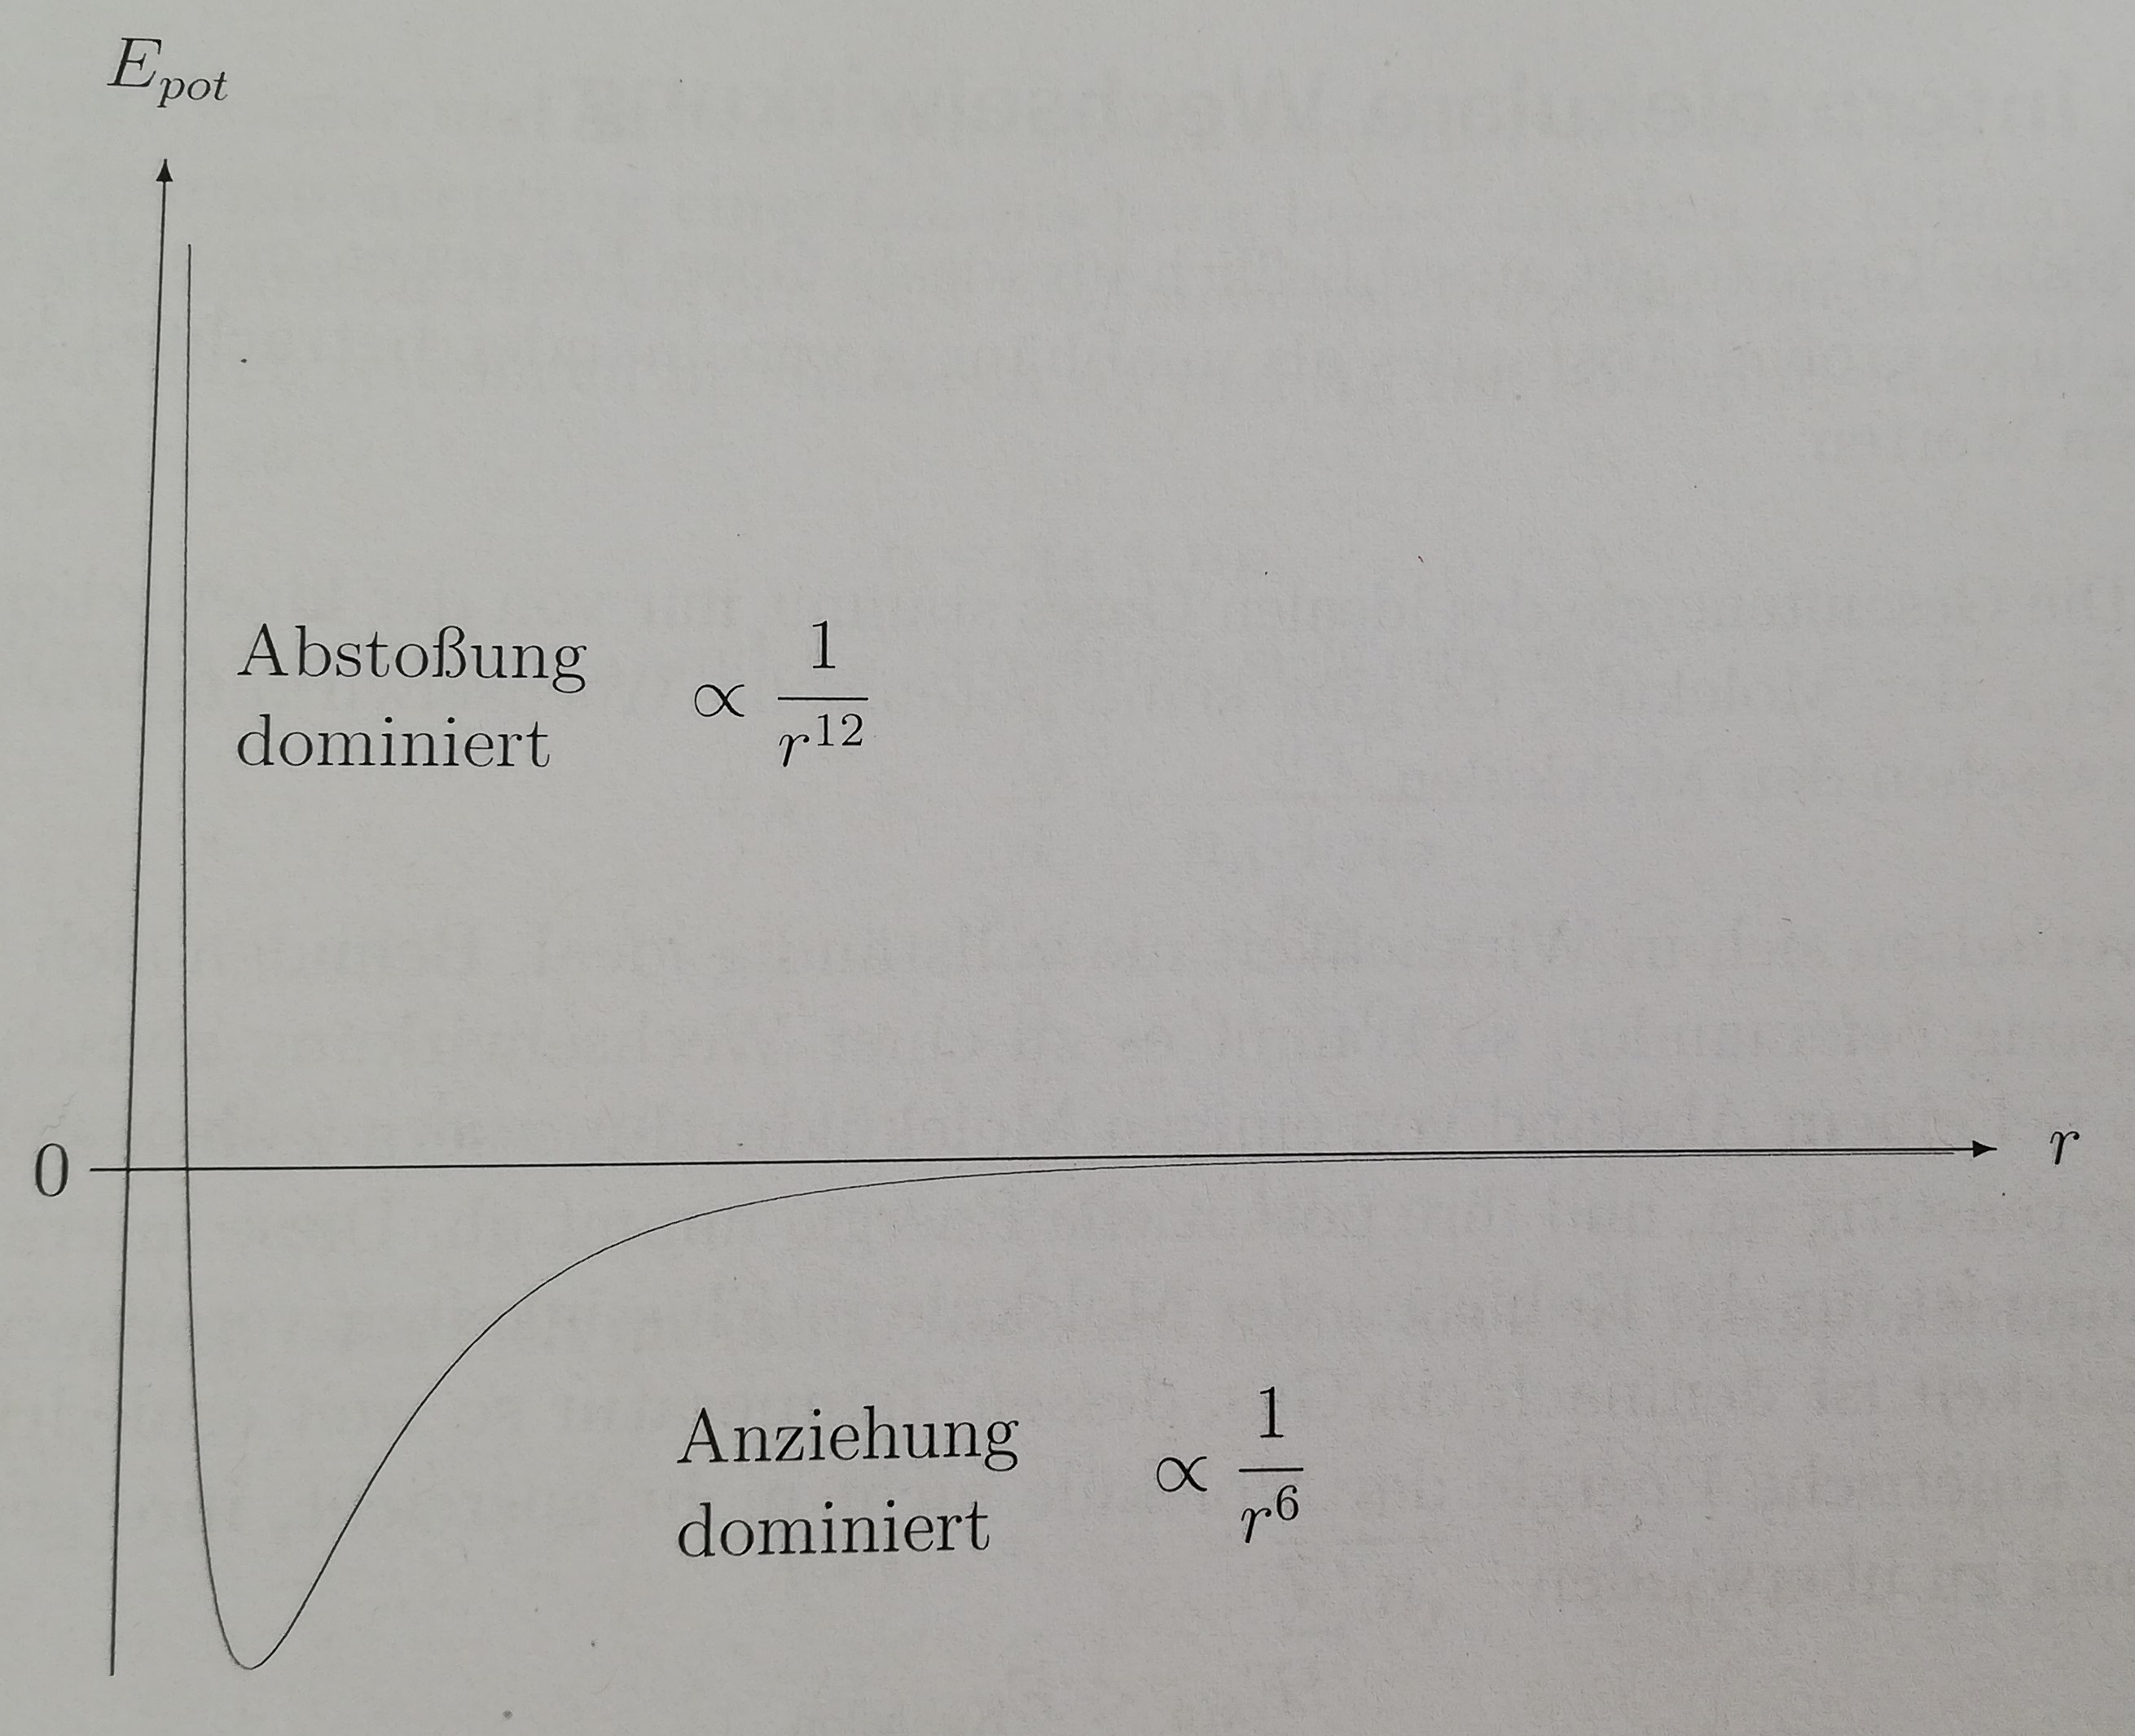
\includegraphics[scale = 0.135]{Bilder/LennardJones.jpg}
    \caption{Skizze des Lennard-Jones-Potentials \protect \footnotemark}
    \label{bild:LJP}
\end{figure}
\footnotetext{\cite{Haefner2019}, S.94}

Diese Wechselwirkungen üben eine Kraft auf den Cantilever aus, der sich infolgedessen verbiegt. Diese Verbiegung wird über einen 
Laserstrahl detektiert, der auf den Cantilever gerichtet ist. Verbiegt sich dieser, so wird auch der Strahl des Lasers unter einem anderen 
Winkel abgelenkt, was ausgewertet werden kann (\cite{Haugstad2012}, S.5). Ein schematischer Aufbau ist in Abb. \ref{bild:Aufbau} zu sehen.

\begin{figure}[h]
    \centering
    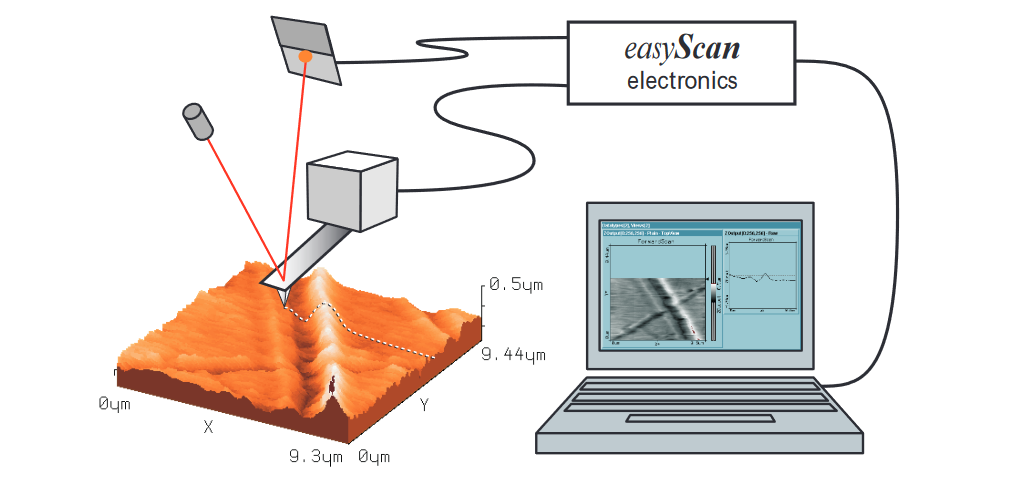
\includegraphics[scale = 0.45]{Bilder/AufbauAFM.png}
    \caption{Schematischer Aufbau eines Rasterkraftmikroskops \protect \footnotemark}
    \label{bild:Aufbau}
\end{figure}
\footnotetext{\cite{easyScan2003}, S.6}

Duch das Funktionsprinzip über die Detektion von wechselwirkungen sind bei der AFM auch keine besonderen Anforderungen an die Probe 
gestellt. Sie müssen insbesondere nicht leitfähig oder im Vakuum sein. \footnotemark \, Dennoch sollten sie frei vor Verunreinigungen sein 
und vor Feuchte geschützt werden; zudem sollte die Probe zu der verwendeten Spitze passen. \\
\footnotetext{Eine AFM im Vakuum liefert dennoch bessere Ergebnisse; für die meisten Zwecke ist eine Untersuchung an der Luft aber 
vollkommen ausreichend}


\newpage


\section{Verwendete Modi}
\label{sec:Modi}
Bei der AFM gibt es einige Betriebsmodi; die im Versuch verwendeten sollen hier kurz erläutert werden.

\subsection{Contact Mode}
Im Contact Mode hat die Spitze des Cantilevers dauerhaft Kontakt mit der zu untersuchenden Probe. Man unterscheidet dabei wiederum zwei Modi: \\
Der Constant Hight Mode ist der einfachster aller Modi. In diesem wird der Cantilever auf einer konstanten Höhe über die Probe gefahren. 
Eine Regelung ist nicht nötig. \footnotemark \\
Im Constant Force Mode wird nicht die Höhe über der Probe, sondern die Kraft, die auf die Spitze wirkt, konstant gehalten. Diese wird 
über den sog. Setpoint eingestellt. Zur Beibehaltung der Kraft ist ein PID-Regler notwendig. (\cite{Rieger2013}, S.8)\\
\footnotetext{\url{https://www.nanosurf.com/en/support/afm-modes-overview/contact-modes}, Stand: 23.09.21}
Obwohl der Contact Mode leicht zu realisieren ist, hat er einige Nachteile. So ist durch den dauerhaften Kontakt die Abnutzung der Spitze 
vergleichsweise hoch; zudem kann diese bei plötzlichen Erhebungen oder schlecht gewählten Einstellungen leicht abbrechen. (\cite{Vesely2017}, S.26)

\subsection{Non-Contact Mode}
Im Non-Contact- oder Tapping-Mode (je nachdem ob die Spitze die Probe nie berührt oder kurz antippt) wird der Cantilever mit einer 
konstanten Frequenz nahe seiner Resonanzfrequenz zum Schwingen angeregt. Diese wird wieder über einen PID-Regler gehalten. 
Die Wechselwirkungen zwischen Probe und Spitze bewirken zum einen eine Änderung der Schwingungsamplitude, über die topographische 
Erkenntnisse gewonnen werden können. (\cite{Vesely2017}, S.26). Zum anderen ergibt sich auch eine Phasenverschiebung, die dazu genutzt 
werden kann, Eigenschaften der Probe zu bestimmen (Dichte etc.). \footnotemark
\footnotetext{\url{https://www.nanosurf.com/en/support/afm-modes-overview/dynamic-modes}, Stand: 23.09.21}
 
\section{Regler}

Regler oder Regelkreise sind wichtige Bestandteile von vielen Messapparaturen. Dabei ist ein Regler im Allgemeinen ein Objekt, welches 
ein Eingangssignal $V_e$ aufnimmt, dieses auf eine Art verarbeitet und dann ein Ausgangssignal $V_a$ ausgibt. Das Eingangssignal könnte 
beispielsweise ein Signal eines Sensors sein und das Ausgangsignal könnte der Steuerung eines Bauelements dienen. Dabei gibt es klassisch einige Elemente, die 
oft in Reglern enthalten sind. Diese heißen auch 'Glieder'.

\subsection*{P-Glied}

Ein P-Glied ist etwas ähnliches wie ein Schalter. Wenn eine bestimmte Bedingung erfüllt ist, dann gibt er einen konstanten Wert aus. Er antwortet also mit einer 
Sprungantwort. Die Antwort ist instantan. Alleine ist er in seiner Anwendung sehr begrenzt; kombiniert man ihn aber mit anderen Gliedern wie dem I- oder D-Glied ist dieser hoch wirksam.

\subsection*{I-Glied}

Das 'I' im Namen kommt von 'Integrieren'. Dabei tut diese Glied genau das, was der Name verspricht. Das I-Glied gibt ein Ausgangssignal aus, welches 
proportional ist zur Integration über das Eingangssignal. Dabei ist klar, dass dieses Glied verzögert antwortet zu dem Eingangssignal, weil 
es dauert bis das Integral entsprechend groß ist.

\subsection*{D-Glied}

Das D-Glied hat nahezu entgegengesetzte Eigenschaften zum I-Glied. Da es als Ausgangsignal ein Signal ausgibt, welches proportional zu Ableitung des 
Eingangssignal ist, reagiert das Glied instantan. Damit kann es Prozesse wie das Einschwingen von langsam reagierenden Elementen verhindern.

\subsection*{Mehrere Glieder}

Oft verwendet man mehrere Glieder additiv, da diese gegenseitig ihr Vorteile zur Geltung bringen. Man sollte jedoch bedenken, dass zu viele Glieder auch das 
Optimieren des Regler erschweren, da es sehr viele Parameter gibt, die angepasst werden müssen.


\section{Faltung und das AFM}

Generell kann man eine Faltung mit der Formel 

\begin{equation*}
    (f \circledast g)(t) = \int_{\-\infty}^\infty f(\tau)g(t-\tau) d\tau
\end{equation*}
berechnen. Sie lässt sich aber auch grafisch berechnen, indem man die eine Funktion nimmt, an der y-Achse spiegelt und dann übereinander 'schiebt'. 
Die Überlappung der beiden Funktionen ist dann das Ergebnis der Faltung. \\

Die Faltung spielt in vielen Bereichen der Physik eine Rolle, auch beim AFM. Das was man misst, ist eine Faltung der Spitzenform mit der realen Probenoberfläche\footnote{\url{https://www.weizmann.ac.il/Chemical_Research_Support/surflab/peter/condecon/index.html}, Aufgerufen: 5.10.2021}. 
Dies ist insofern auch schlüssig, da man so keine 'Spalten' in der Probe sehen kann, die schmaler als die Spitze sind. Das gleiche Ergebnis erhält man, wenn man Faltet, da die Faltung 
zweier Funktionen runder ist als die rundere der beiden Funktionen.